\chapter{Identidad gráfica}

Hasta ahora, las inspiraciones para la revista han sido \href{https://www.pentagram.com/work/scientific-american?rel=sector&rel-id=3}{un rediseño de la revista Scientific American}, la revista \href{https://www.frontiersin.org/journals/sustainability/articles/10.3389/frsus.2026.1818134/pdf}{Frontiers}, \href{https://www.sciencedirect.com/science/article/pii/S1198743X26000650/pdfft?pid=1-s2.0-S1198743X26000650-main.pdf}{Elsevier} y algunas ideas en \href{https://pin.it/3s68QTUbZ}{Pinterest}.

Si bien aún pueden realizarse mejoras, se esperará a recibir retroalimentación de docentes y alumnos para aplicarlas. Asímismo, en un futuro también se aceptarán recomendaciones de alumnos y docentes para mejorar el diseño de la revista.

\section{Paleta de colores}

La paleta de colores utilizada en la revista está inspirada en los colores institucionales de UPSIN. A continuación se listan los colores utilizados en la revista y las áreas en que se usa cada uno:

    \begin{figure}[H]
    \centering
    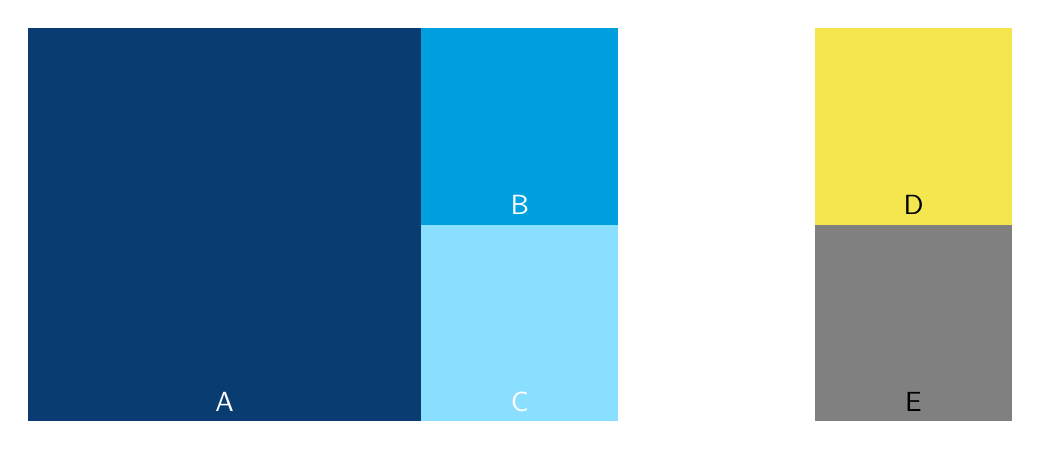
\begin{tikzpicture}
        \fill[Primario] (0,0) rectangle (5,5);
            \node[anchor=south,font=\sffamily\selectfont,white] at (2.5,0) {A};

        \fill[Acento] (5,0) rectangle (7.5,2.5);
            \node[anchor=south,font=\sffamily\selectfont,white] at (6.25,0) {C};
        \fill[Secundario] (5,2.5) rectangle (7.5,5);
            \node[anchor=south,font=\sffamily\selectfont,white] at (6.25,2.5) {B};

        \fill[Grey] (10,0) rectangle (12.5,2.5);
            \node[anchor=south,font=\sffamily\selectfont,black] at (11.25,0) {E}; 
        \fill[Complemento] (10,2.5) rectangle (12.5,5);
            \node[anchor=south,font=\sffamily\selectfont,black] at (11.25,2.5) {D};
    \end{tikzpicture}
    \rule{\linewidth}{0.2pt}
    \caption{Paleta de colores}
    \label{fig:paleta_de_colores}
\end{figure}

        \definecolor{Primario}{RGB}{9,60,113}
        \definecolor{Secundario}{RGB}{0,160,224}
        \definecolor{Acento}{RGB}{138,222,255}
        \definecolor{Complemento}{RGB}{245,230,80}

\begin{itemize}
    \item Color principal (A) - RGB(9,60,113)
        \subitem Contador de tablas y figuras (Tabla X, Figura X)
        \subitem Color de fondo para encabezado en tablas a una columna
        \subitem Enlaces externos
    \item Color secundario (B) - RGB(0,160,224)
        \subitem Enlaces internos (citas, figuras y tablas)
    \item Color de acento (C) - RGB(138,222,255)
    \item Color de complemento (D) - RGB(245,230,80)
    \item Gris (E) - RGB(242,242,242)
        \subitem Color de fondo para filas en tablas (intercalado con blanco)
\end{itemize}

\section{Tipografías}

Se estarían utilizando 2 tipografías: Red Hat Display y Crimson Pro. Cada una sería utilizada en diferentes  áreas.

La tipografía Red Hat Display (\autoref{fig:tipografía_red_hat_display}) sería utilizada para titulos y encabezados, variando y combinando su estilo y peso (negrita, normal e itálica) para cada nivel de titulo o encabezado. También se estaría utilizando para los contadores de figuras y tablas (Tabla X, Figura X).

    \vspace{1em}
\begin{figure}[H]
    \centering
    {\sffamily\LARGE\selectfont \textbf{AaBbCc} \quad  AaBbCc \quad \textit{AaBbCc}}
    \vspace{1em}
    \textcolor{Primario}{\rule{\linewidth}{0.2pt}}
    \vspace*{-2em}
    \caption{Tipografía Red Hat Display (Negritas, normal e itálica)}
    \label{fig:tipografía_red_hat_display}
\end{figure}

Por otro lado, la tipografía Crimson Pro (\autoref{fig:tipografía_crimson_pro}) sería utilizada para el texto principal, así como descripciones de tablas y figuras.

    \vspace{1em}
\begin{figure}[H]
    \centering
    {\LARGE\selectfont \textbf{AaBbCc} \quad  AaBbCc \quad \textit{AaBbCc}}
    \vspace{1em}
    \textcolor{Primario}{\rule{\linewidth}{0.2pt}}
    \vspace*{-2em}
    \caption{Tipografía Crimson Pro (Negritas, normal e itálica)}
    \label{fig:tipografía_crimson_pro}
\end{figure}


Para el texto general se utilizará un tamaño de 12pt. Para los encabezados de distintos niveles se utilizarán los siguientes tamaños:

\begin{itemize}
    \item 18pt en negritas 
    \item 16pt en negritas
    \item 14pt en itálica
\end{itemize}

\section{Presentación de tablas y figuras}

\subsection{Tablas}

Los encabezados de las tablas tendrán Red Had Display como tipografía, mientras que el resto de la tabla (cuerpo y notas a pie) mantendrán Crimson Pro como tipografía.

El color de las filas del cuerpo alternará entre blanco y gris. En el caso de los encabezados estos podrán utilizar el color primario (azul oscuro, \autoref{tab:ejemplo_tabla_azul}) o blanco como color de fondo (\autoref{tab:ejemplo_tabla_blanco}).

    \newpage

\begin{multicols}{2}

\begin{table}[H]

\caption{Ejemplo de tabla con encabezados color azul}
\label{tab:ejemplo_tabla_azul}

\begin{threeparttable}

{\small\setstretch{1.35}\rowcolors{1}{Grey}{White}

\begin{tabular}{M{0.4\linewidth}M{0.4\linewidth}}\hline
    
    \sffamily\bfseries\cellcolor{Primario}\textcolor{White}{Encabezado 1} & \sffamily\bfseries\cellcolor{Primario}\textcolor{White}{Encabezado 2} \\ \hline
    
    Dato 1 & Dato 2\tnote{1} \\
    Dato 3 & Dato 4 \\
    Dato 5 & Dato 6 \\
    Dato 7 & Dato 8 \\

    \hline
\end{tabular}

}

\begin{tablenotes}\tiny % ex: \tnote{1} ... \item[1]
    \item[1] Ejemplo de nota a pie de tabla
\end{tablenotes}

\end{threeparttable}
\end{table}



\begin{table}[H]

\caption{Ejemplo de tabla con encabezados color blanco}
\label{tab:ejemplo_tabla_blanco}

\begin{threeparttable}

{\small\setstretch{1.35}\rowcolors{1}{Grey}{White}

\begin{tabular}{M{0.4\linewidth}M{0.4\linewidth}}\hline
    
    \sffamily\bfseries\cellcolor{White}\textcolor{Primario}{Encabezado 1} & \sffamily\bfseries\cellcolor{White}\textcolor{Primario}{Encabezado 1} \\ \hline
    
    Dato 1 & Dato 2\tnote{1} \\
    Dato 3 & Dato 4 \\
    Dato 5 & Dato 6 \\
    Dato 7 & Dato 8 \\

    \hline
\end{tabular}

}

\begin{tablenotes}\tiny % ex: \tnote{1} ... \item[1]
    \item[1] Ejemplo de nota a pie de tabla
\end{tablenotes}

\end{threeparttable}
\end{table}

\end{multicols}

\subsection{Figuras}

En el caso de las figuras se respetará el diseño de los autores originales. Se usará una linea azul oscuro para separar la figura de la descripción.

\begin{figure}[H]
    \centering
    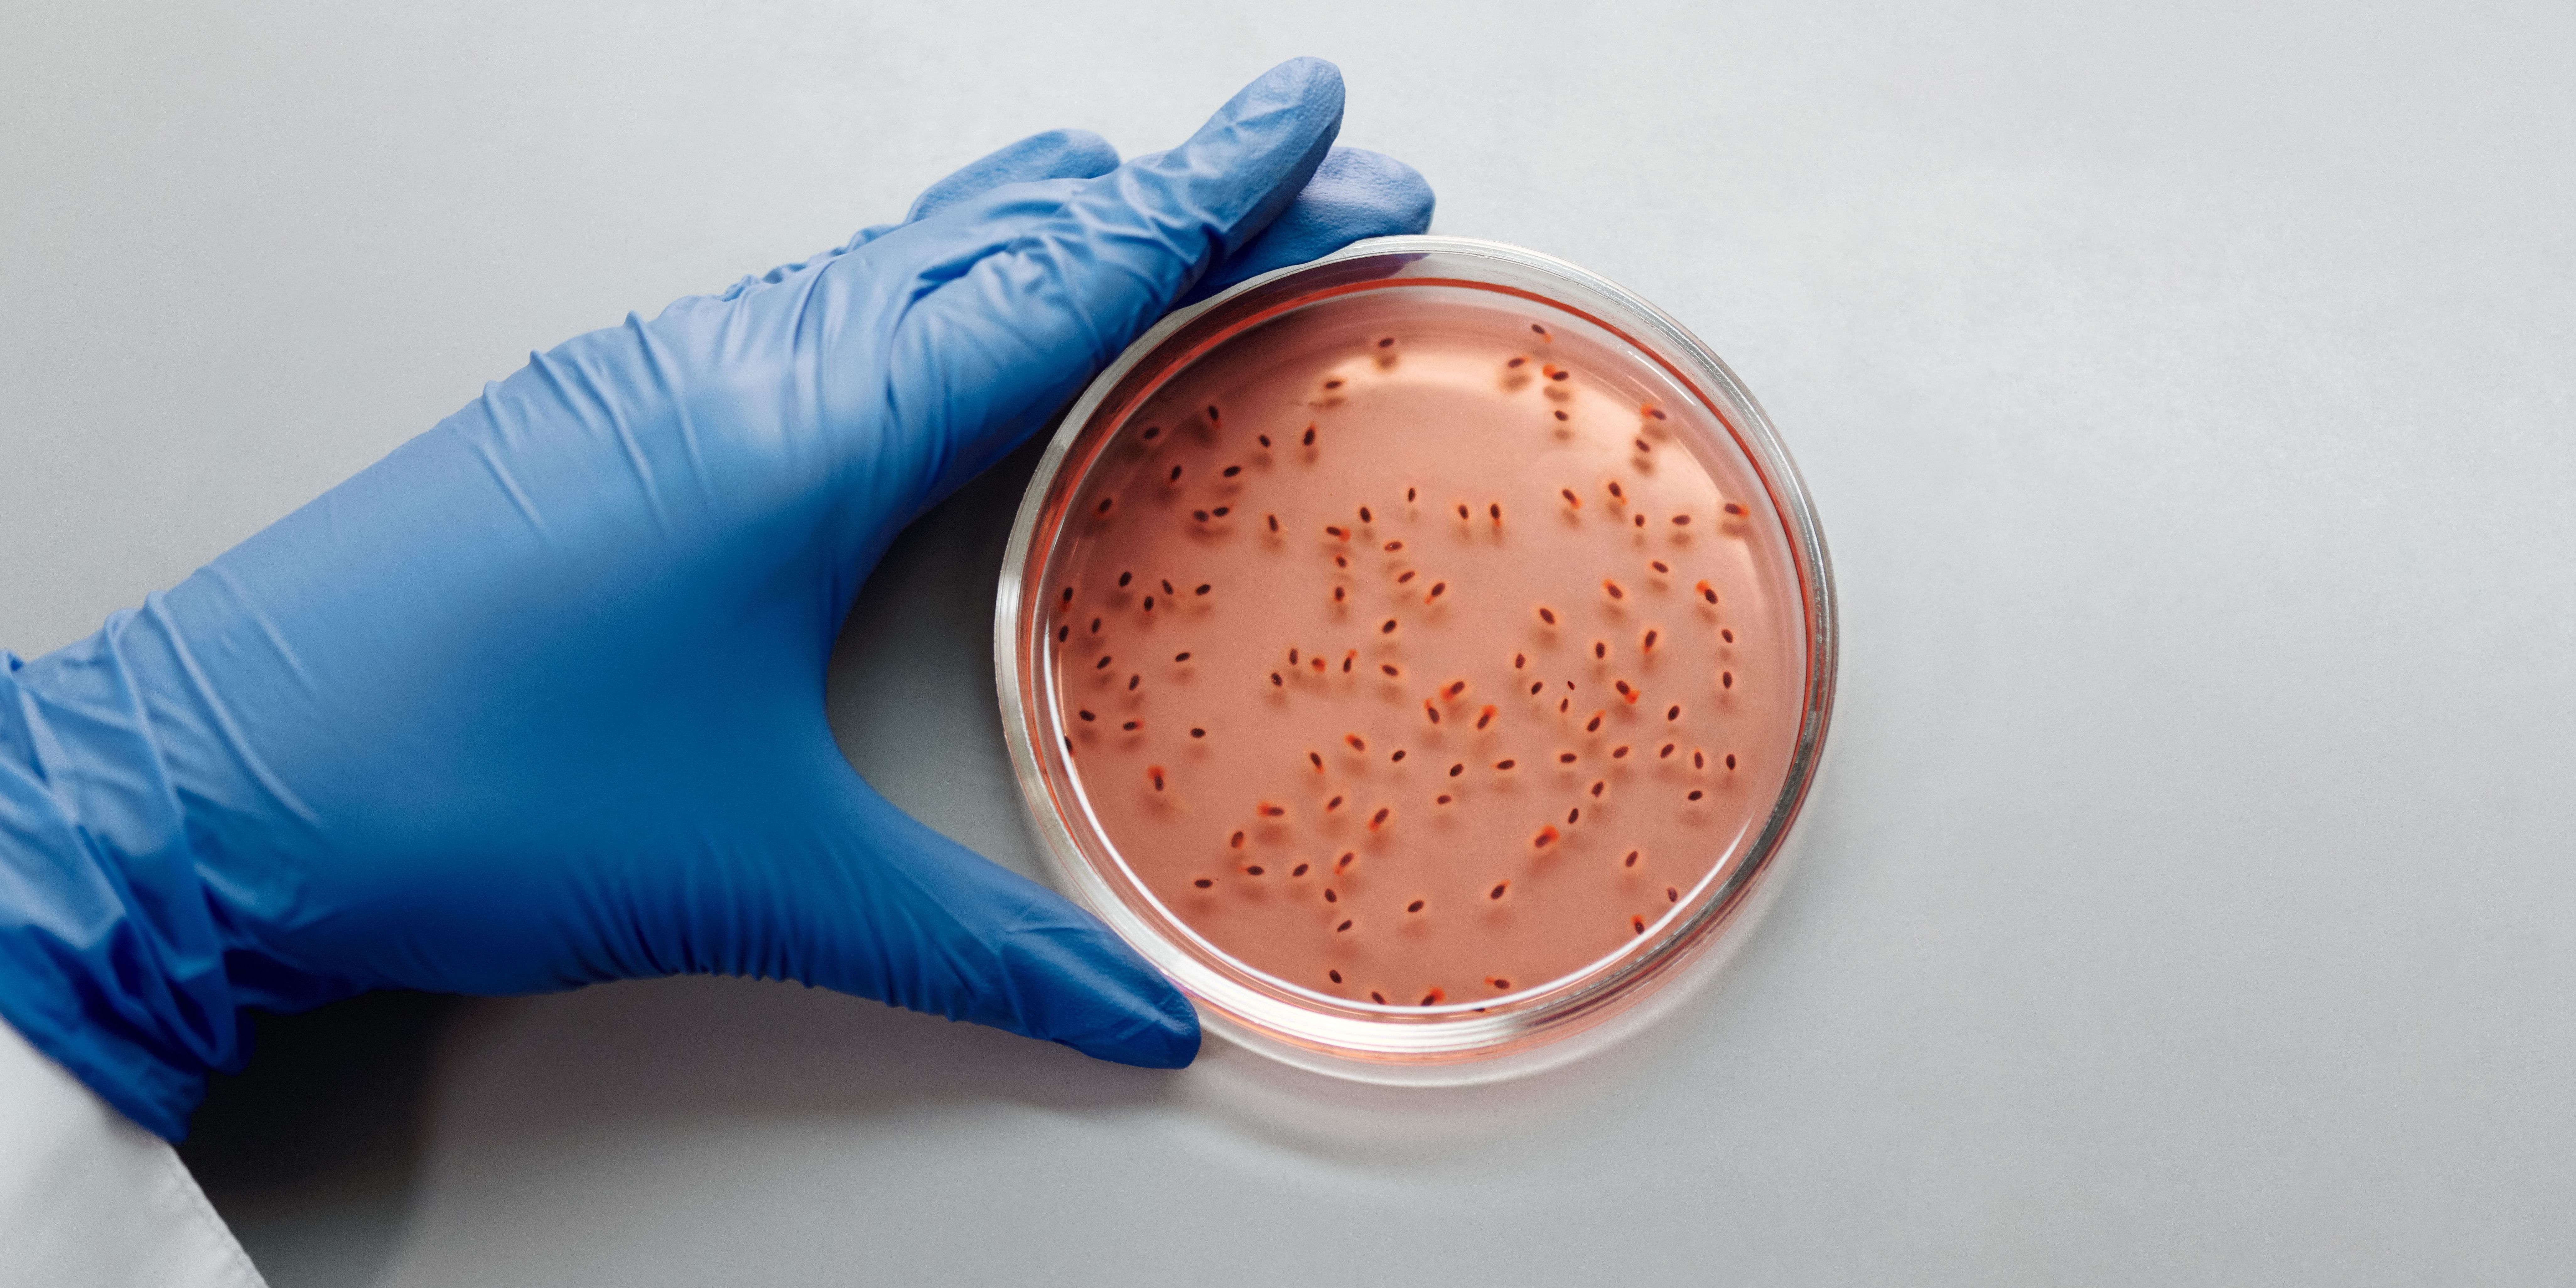
\includegraphics[width=0.85\linewidth]{fig:ejemplo_figura}
    \textcolor{Primario}{\rule{\linewidth}{0.2pt}}
    \caption{Ejemplo de figura}
    \label{fig:ejemplo_figura}
\end{figure}